\documentclass[../interim.tex]{subfiles}


\begin{document}

\chapter{Project Plan}

In order to provide a plan of the work to be completed, this chapter firstly describes what has been achieved so far, provides possible solutions to some of the key problems which need to be solved and outlines possible methods for evaluating the performance of a completed system.

\section{Completed Work}

Many VideoQA datasets were outlined in the related work discussion in Chapter~\ref{chapter:related}. However, these pre-existing datasets do not contain the semantic information required to extract symbolic properties from objects in each frame. Most of these datasets provide nothing more than a sequence of images, a question and an answer. While this is sufficient to train an end-to-end neural network, since it learns implicit features, it does not allow us to train a network which can extract explicit object properties, which are required for logical reasoning. Although it would be possible to extract some information using a network pre-trained on ImageNet~\cite{imagenet}, for example, we would only be able to extract bounding boxes and classes for each object, whereas we would prefer to extract richer details such as colour, rotation or size. Furthermore, we cannot guarantee that every object in a scene is part of the ImageNet dataset, therefore it would be possible for a network to miss some objects entirely.

For this reason we have decided to generate a dataset which provides the information needed for logical reasoning, as a starting point for building our model. The dataset emulates a simple retro game environment. Since the focus of this project is to investigate logical reasoning and the learning of symbolic rules, we do not attempt to make the job of the neural network difficult by creating very complex scenes; each frame is very simple with a flat background and no variation in object shape. Each image is also quite small at only 128x128 pixels, which will allow for faster network training.

An example sequence of frames from the current version of the dataset is shown in Figure~\ref{fig:dataset-frames}.

\begin{figure}[ht!]
  \begin{subfigure}{0.24\textwidth}
    \centering
    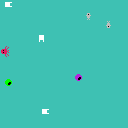
\includegraphics[width=\textwidth]{frame_1.png}
  \end{subfigure}
  \hfill
  \begin{subfigure}{0.24\textwidth}
    \centering
    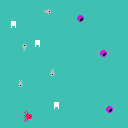
\includegraphics[width=\textwidth]{frame_2.png}
  \end{subfigure}
  \hfill
  \begin{subfigure}{0.24\textwidth}
    \centering
    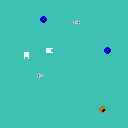
\includegraphics[width=\textwidth]{frame_3.png}
  \end{subfigure}
  \hfill
  \begin{subfigure}{0.24\textwidth}
    \centering
    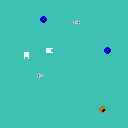
\includegraphics[width=\textwidth]{frame_4.png}
  \end{subfigure}
  \caption{An example sequence of frames from the initial version of the dataset.}
  \label{fig:dataset-frames}
\end{figure}

The key elements of the dataset are the following:
\begin{itemize}
  \item \textbf{Octopus}. The `main' character in the frames - the octopus is the only character which moves and its properties change as it comes into contact with other objects.

  \item \textbf{Fish}. The fish are always silver, but can have any rotation. When the octopus comes close to the fish, the fish disappears (gets eaten).

  \item \textbf{Plastic Bag}. Similarly to the fish, the plastic bags are always white but can have any rotation. Each bag is harmful to the octopus, so both objects disappear when in close contact.

  \item \textbf{Rock}. Rocks can have four colours: brown, blue, purple and green, but always face upright. While an octopus is near a rock the octopus' colour will match that of the rock (it will be camouflaged).
\end{itemize}

The idea behind the dataset is to show object property changes which have well-defined semantics that are non-trivial to learn. For example, given the location and colour of objects from two successive frames, we would like to investigate whether ILASP could learn that the octopus only changes colour when it is close to a rock (and what exactly it means to be close). At the moment we only have a very early version of the dataset and we may well be required to add more objects with more complex semantics in later stages of the project. In later versions of the dataset we also intend to provide information on the events which occur between frames, but this has not yet been included.

Each object in each frame is labelled with the following information:
\begin{itemize}
  \item \textbf{Class}. The object type, as described above.

  \item \textbf{Bounding Box}. We provide the upper left and lower right coordinates of the box around the object.

  \item \textbf{Colour}. The current colour of the object.

  \item \textbf{Rotation}. The compass direction the object is currently facing in. This is given as an integer between 0 and 3.
\end{itemize}

\section{Implementation Plan}

In Chapter~\ref{chapter:intro} we outlined four key challenges that we think will need to solved in order to build a functioning hybrid VideoQA model. We now describe our initial ideas for how these can be overcome:
\begin{enumerate}
  \item \textbf{Object Detection}. A number of models exist for this task, as shown in Chapter~\ref{chapter:background}. We propose to adapt one of these models to fit our own dataset and train it to be capable of producing bounding boxes and class labels for each object in a frame.

  \item \textbf{Property Extraction}. Now that we have access to a dataset with the required object information, we can simply build a neural network which takes the output of the \textit{object detection} step and produces the required properties of the object. It may also be interesting to investigate whether this network can be directly combined with the object detection network, classifying each property in the same way as the object class.

  \item \textbf{Event Detection}. Earlier we outlined a number of object tracking methods that can be used to track multiple objects through frames simultaneously. We could compare the performance differences between using motion and appearance features for this task. Once we have a working object tracker we will need to use it to classify an event between two frames. To start with, we could assume we are given an $\mathcal{AL}$ system description of the environment and write an ASP program which, when given the properties extracted from two successive frames, classifies an event between those frames. Building on this, we could investigate ways to use the event information provided in the dataset to train neural networks to do some of this classification for us. This may also require the use of ILASP, since we may not be able to ask a network to predict which objects were involved in an event when there are an arbitrary number of objects.

  \item \textbf{Question and Knowledge Representation}. We will need to investigate ways of representing the question in ASP in a form that, when given the information from the video, allows us to find an answer. This will probably require creating templates for questions and answers. In the later stages of the project it may also be interesting to investigate how we could learn $\mathcal{AL}$ descriptions using ILASP, rather than assume them.
\end{enumerate}

From the challenges described above, we outline the following set of milestones in the development of a working hybrid VideoQA model:
\begin{enumerate}
  \item Construct an initial dataset of videos (QA pairs not required at this stage).

  \item Build neural network(s) for object detection and property extraction, and train them on the constructed dataset.

  \item Investigate different object tracking methods and build an algorithm that, when given the object properties for each frame, can assign the properties to specific objects using an appropriate tracking method.

  \item Write an ASP program which, when given an $\mathcal{AL}$ system description encoding and object properties for each frame, classifies an event between two frames.

  \item Construct a dataset enriched with templated questions and answers, and find a way to encode the questions in ASP.

  \item Build a complete VideoQA model which makes use of the above algorithms to find the required answer to a question when given a sequence of frames.
\end{enumerate}

It is possible that some of these milestones may prove to be too challenging within the timeframe. However, since most of the above milestones are stand-alone, progress can still be made in other areas. It is also the case that some subcomponents can be created artificially. For example, if the neural networks did not work, we could simply provide the correct output in order to test the rest of the system.

After building a working hybrid VideoQA model, a key extension for the project would be to remove as much prior information about the environment as possible. This could mean trying to learn $\mathcal{AL}$ system descriptions, removing the additional semantic information from the dataset (and only working with bounding boxes and class labels), or ditching question templates in favour of free-form questions and answers.

With this in mind, we outline the following possible extensions to the VideoQA model which would, in theory, allow it operate on other VideoQA datasets:
\begin{itemize}
  \item Remove prior $\mathcal{AL}$ encodings of the environment and investigate the possibility of using ILASP to learn the system description instead. It will also be necessary to find another method for classifying events, since we cannot use $\mathcal{AL}$ system descriptions. Neural networks may be helpful, but it would be preferable to avoid adding event labels to the dataset.

  \item Remove additional object property labels from the dataset and work with bounding boxes and classes alone, as this would better emulate the information provided by an object detection dataset. Some form of unsupervised learning may be heplful for this, and making use of the information provided by the answers to questions will almost certainly be required.

  \item Investigate ways of encoding the information provided by free-form questions and asnwers in ASP. This could make the model much more applicable to pre-existing VideoQA datasets but is probably a research project in its own right.

  \item Investigate adding additional layers of difficulty to the dataset. For example, we could allow non-deterministic actions, or other external events with more complex semantics.
\end{itemize}

\section{Evaluation Plan}

Finally, this section outlines some evaluation strategies which could help to provide an insight into the performance of our model.

Firstly, throughout model construction we will want to ensure that each subcomponent is performing well. For this reason, it will be useful to compare quantitatively possible subcomponent implementations. For example, we will want to compare different object tracking methods, as well different neural network implementations. The metrics described in Chapter~\ref{chapter:background} will he helpful for this.

When we have a complete model we can use traditional VideoQA metrics, such as accuracy, to evaluate its performance. To do this we will firstly need to split the dataset into training and testing subsets, and ensure that none of the testing data is used for training or tuning the model. We can then apply the testing data to the model and record the number of correct and incorrect answers. It may also be helpful to train some of the end-to-end VideoQA models on our dataset and compare their performance to ours. It is worth noting, however, that, because it makes use of the templates for questions, our model has a significant advantage over any model which does not use this pre-defined information. We could still use these evaluations as baselines.

Finally, after building and evaluating our VideoQA model, it may be interesting to investiage how its performance degrades as we artificially alter the performance of individual components. It may be the case that by having a pipelined model, such as ours, with multiple learning components, the overall model performance is not severely affected by a single underperforming component.


\end{document}
